\documentclass[
	% -- opções da classe memoir --
	12pt,				% tamanho da fonte
	openright,			% capítulos começam em pág ímpar (insere página vazia caso preciso)
	oneside,			% para impressão em verso e anverso. Oposto a oneside
	a4paper,			% tamanho do papel. 
	% -- opções da classe abntex2 --
	%chapter=TITLE,		% títulos de capítulos convertidos em letras maiúsculas
	%section=TITLE,		% títulos de seções convertidos em letras maiúsculas
	%subsection=TITLE,	% títulos de subseções convertidos em letras maiúsculas
	%subsubsection=TITLE,% títulos de subsubseções convertidos em letras maiúsculas
	% -- opções de sumário -- %
	sumario=abnt-6027-2012, % sumário conforme as recomendações da ABNT NBR 6027:2012 (padrão)
	%sumario=tradicional, % usa o estilo tradicional de sumários do memoir
	.
	% -- opções do pacote babel --
	english,			% idioma adicional para hifenização
	brazil				% o último idioma é o principal do documento
	]{abntex2}


% --- 
% CONFIGURAÇÕES DE PACOTES
% --- 
% ---
% Pacotes básicos 
% ---
\usepackage{lmodern}			% Usa a fonte Latin Modern			
\usepackage[T1]{fontenc}		% Selecao de codigos de fonte.
\usepackage[utf8]{inputenc}		% Codificacao do documento (conversão automática dos acentos)
\usepackage{lastpage}			% Usado pela Ficha catalográfica
\usepackage{indentfirst}		% Indenta o primeiro parágrafo de cada seção.
\usepackage{color}				% Controle das cores
\usepackage{graphicx}			% Inclusão de gráficos
\usepackage{microtype} 			% para melhorias de justificação
\usepackage{ufc-abntex2}

\usepackage{amsmath}            % Organizar numeração das figuras por seção 
\numberwithin{figure}{chapter}

 \usepackage{tikz}
 \usetikzlibrary{mindmap}
 \usepackage{metalogo}
% \usepackage{dtklogos}

%\usepackage{subfig}
% ---
		
% ---
% Pacotes adicionais, usados apenas no âmbito do Modelo Canônico do abnteX2
% ---
\usepackage{lipsum}				% para geração de dummy text
\usepackage[nolist]{acronym}    % Inclusão de acronimos
% ---

% ---
% Pacotes de citações
% ---
\usepackage[brazilian,hyperpageref]{backref}	 % Paginas com as citações na bibl
\usepackage[alf,abnt-and-type=e,abnt-full-initials=no,abnt-last-names=abnt,abnt-etal-list=2,abnt-etal-text = emph,abnt-emphasize=bf]{abntex2cite}
%\usepackage[alf]{abntex2cite}	% Citações padrão ABNT

% ---
% Configurações do pacote backref
% Usado sem a opção hyperpageref de backref
\renewcommand{\backrefpagesname}{Citado na(s) página(s):~}
% Texto padrão antes do número das páginas
\renewcommand{\backref}{}
% Define os textos da citação
\renewcommand*{\backrefalt}[4]{
	\ifcase #1 %
		Nenhuma citação no texto.%
	\or\renewcommand{\cftsubsectionfont}{\bfseries\itshape}
	\renewcommand{\cftsubsubsectionfont}{\bfseries}
	
		Citado na página #2.%
	\else
		Citado #1 vezes nas páginas #2.%
	\fi}%
% ---

% ---
% Configurações de aparência do PDF final

%\renewcommand{\cftsubsectionfont}{\bfseries\itshape}
\renewcommand{\cftsubsectionfont}{\itshape}
\renewcommand{\cftsubsubsectionfont}{\itshape}
\renewcommand{\cftsubsubsectionfont}{\cftsubsectionfont}

\newcommand\figref{Figura~\ref}
\newcommand\capref{Capítulo~\ref}
\newcommand\tabref{Tabela~\ref}
\newcommand\secref{Seção~\ref}
% alterando o aspecto da cor azul
\definecolor{blue}{RGB}{41,5,195}

% informações do PDF
\makeatletter
\hypersetup{
     	%pagebackref=true,
		pdftitle={\@title}, 
		pdfauthor={\@author},
    	pdfsubject={\imprimirpreambulo},
	    pdfcreator={LaTeX with abnTeX2},
		pdfkeywords={abnt}{latex}{abntex}{abntex2}{trabalho acadêmico}, 
		colorlinks=true,       		% false: boxed links; true: colored links
    	linkcolor=black,          	% color of internal links
    	citecolor=black,        		% color of links to bibliography
    	filecolor=black,      		% color of file links
		urlcolor=black,
		bookmarksdepth=4
}
\makeatother
% --- 

% Definições matemáticas
\newcommand{\mean}[1]{\mathbb{E}\left\{ #1 \right\}}
\newcommand{\Abs}[1]{\left\vert #1 \right\vert}
\newcommand{\stK}{\Set{K}}
\usepackage{mathtools}
\usepackage{amssymb,amstext,amsfonts}

% Pacote para tabela
\usepackage{threeparttable}

\usetikzlibrary{arrows.meta}
\tikzset{%
	>={Latex[width=2mm,length=2mm]},
	% Specifications for style of nodes:
	base/.style = {rectangle, rounded corners, draw=black,
		minimum width=4cm, minimum height=1cm,
		text centered, font=\sffamily},
	activityStarts/.style = {base, fill=blue!30},
	startstop/.style = {base, fill=red!30},
	activityRuns/.style = {base, fill=green!30},
	process/.style = {base, minimum width=2.5cm, fill=orange!15,
		font=\ttfamily},
}

% Cross reference
\usepackage{xr}
%acro
\usepackage{acronym}

% --- 
% Espaçamentos entre linhas e parágrafos 
% --- 

% O tamanho do parágrafo é dado por:
\setlength{\parindent}{1.3cm}

% Controle do espaçamento entre um parágrafo e outro:
\setlength{\parskip}{0.2cm}  % tente também \onelineskip

% ---
% compila o indice
% ---
\makeindex
% ---
\begin{document}
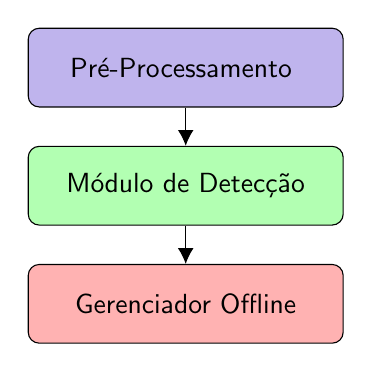
\begin{tikzpicture}[node distance=1.5cm,
every node/.style={fill=white, font=\sffamily}, align=center]
% Specification of nodes (position, etc.)
\node (start)             [activityStarts]              {Pré-Processamento };
%\node (onCreateBlock)     [process, below of=start]          {Entropia de IPs origem,\\ Variação de IPs origem e Taxa de Pacotes};
%\node (onStartBlock)      [process, below of=onCreateBlock]   {onStart()};
%\node (onResumeBlock)     [process, below of=onStartBlock]   {onResume()};
\node (activityRuns)      [activityRuns, below of=start]
{Módulo de Detecção};
%\node (onPauseBlock)      [process, below of=activityRuns, yshift=-1cm]
%{onPause()};
%\node (onStopBlock)       [process, below of=onPauseBlock, yshift=-1cm]
%{onStop()};
%\node (onDestroyBlock)    [process, below of=onStopBlock, yshift=-1cm] 
%{onDestroy()};
%\node (onRestartBlock)    [process, right of=onStartBlock, xshift=4cm]
%{onRestart()};
%\node (ActivityEnds)      [startstop, left of=activityRuns, xshift=-4cm]
%{Process is killed};
\node (ActivityDestroyed) [startstop, below of=activityRuns]
{Gerenciador Offline};     
% Specification of lines between nodes specified above
% with aditional nodes for description 
\draw[->]             (start) -- (activityRuns);
%\draw[->]     (onCreateBlock) -- (onStartBlock);
%\draw[->]      (onStartBlock) -- (onResumeBlock);
\draw[->]     (activityRuns) -- (ActivityDestroyed);
%\draw[->]      (activityRuns) -- node[text width=4cm]
%{Another activity comes in
%	front of the activity} (onPauseBlock);
%\draw[->]      (onPauseBlock) -- node {The activity is no longer visible}
%(onStopBlock);
%\draw[->]       (onStopBlock) -- node {The activity is shut down by
%	user or system} (onDestroyBlock);
%\draw[->]    (onRestartBlock) -- (onStartBlock);
%\draw[->]       (onStopBlock) -| node[yshift=1.25cm, text width=3cm]
%{The activity comes to the foreground}
%(onRestartBlock);
%\draw[->]    (onDestroyBlock) -- (ActivityDestroyed);
%\draw[->]      (onPauseBlock) -| node(priorityXMemory)
%{higher priority $\rightarrow$ more memory}
%(ActivityEnds);
%\draw           (onStopBlock) -| (priorityXMemory);
%\draw[->]     (ActivityEnds)  |- node [yshift=-2cm, text width=3.1cm]
%{User navigates back to the activity}
%(onCreateBlock);
%\draw[->] (onPauseBlock.east) -- ++(2.6,0) -- ++(0,2) -- ++(0,2) --                
%node[xshift=1.2cm,yshift=-1.5cm, text width=2.5cm]
%{The activity comes to the foreground}(onResumeBlock.east);
\end{tikzpicture}	
\end{document}
